\section{Pattern recognition and track fitting approaches}

\subsection{Introduction to associative memory approach}

\noindent Using associative memories in order to perform a fast pattern recognition (PR) at the trigger stage was first exposed in Ref.~\cite{bib:Del-89}. The principle is sketched in Fig.~\cite{fig:AM_principle}:
\begin{figure}[ht!]
\centering
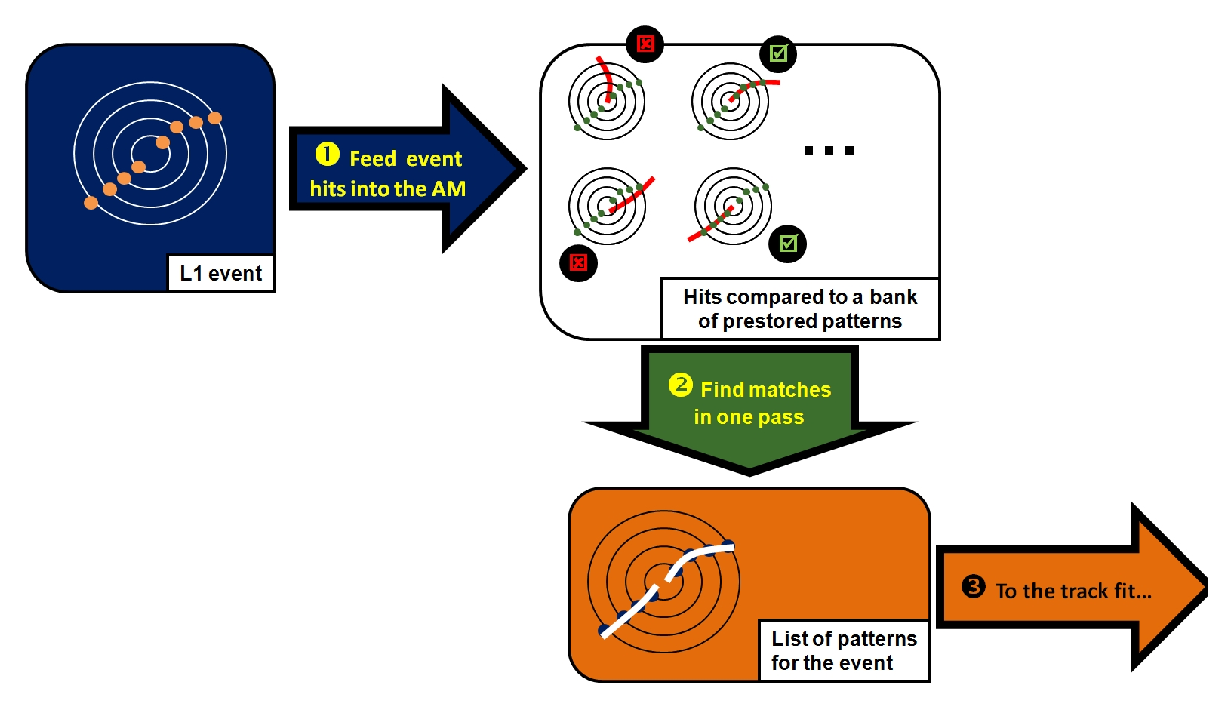
\includegraphics[width=0.7\columnwidth]{Plots/TriggerAM.eps}
\caption{Pattern recognition using associative memories.}
\label{fig:AM_principle}
\end{figure}

\noindent The idea is to compare the hits recorded in the tracking system to a bank of patterns stored in an associative memory chip. The patterns could be seen as low-granularity tracks, they are defined once for all using Monte-Carlo events, and they are ideally covering all the possible tracks occuring in the detector. In this part we will concentrate ourselves on the pattern bank definition. This is indeed the central point of the PR stage. The bank, which is defined using simulated events, has to fulfill few requirements. Before presenting them, it's important to define some parameters. 

\subsection{System configuration}

\subsubsection{Dividing the tracking system into sectors}

\noindent Before defining more precisely the pattern itself, one could introduce a very simple way to reduce the bank size, based on cyclindrical symmetry of the system. Tracker barrels and endcaps could indeed be azimuthally divided into symmetric sectors. The first stage to reduce the bank size will therefore be to generate banks for sectors, not for the whole detector. This doesn't mean that the banks will be exactly identical for all sectors, however, this will reduce the size of the banks to store.

\noindent It is tempting, at this stage, to divide the detector into very small sectors, in order to work with smaller banks. However, the minimal sector size is geometrically constrained by the track trigger requirements. The system should indeed be able to detect tracks over a given $p_T$ threshold (in our case $2~GeV/c$). The minimal sector should thus entirely contain such tracks. The maximum angular deviation of the particles we are looking for is easy to compute.
\begin{figure}[ht!]
\centering
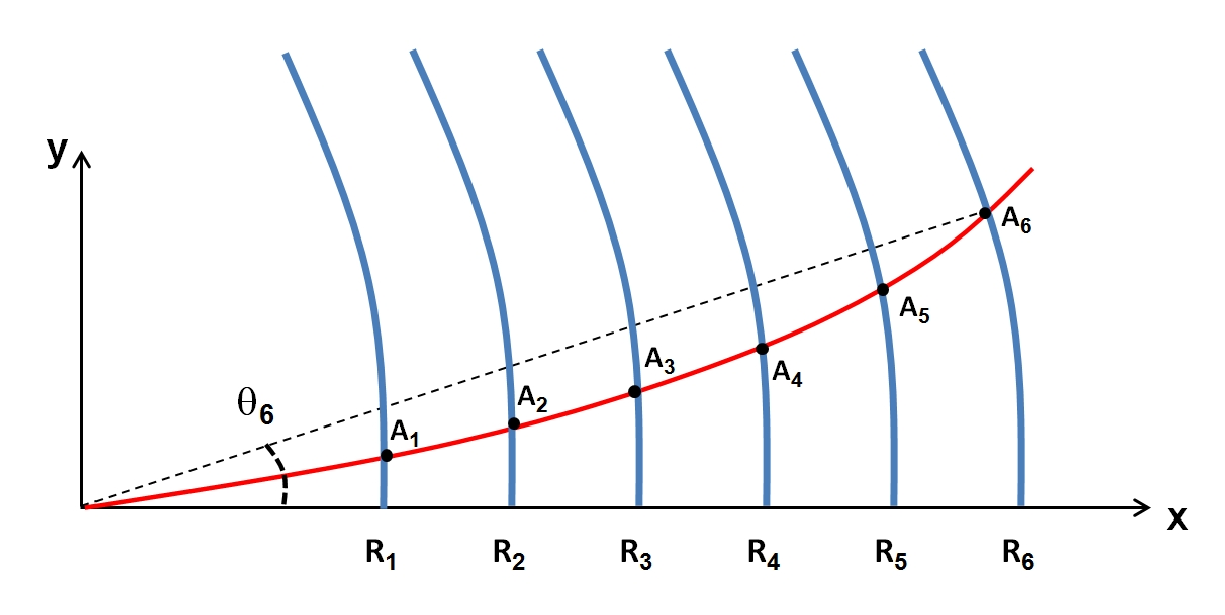
\includegraphics[width=0.6\columnwidth]{Plots/Deviations.eps}
\caption{Particle deviation in the different layers.}
\label{fig:Deviat}
\end{figure}

\noindent Using the notations of Fig.~\ref{fig:Deviat}, and considering that the particle has a curvature $R_c$, and is tangent to the x-axis at origin, one easily gets the coordinates $(x_i,y_i)$ of the points $A_i$, where the particle is crossing the layers (see Sec.~\label{sec:STUB}). The angular deviation is then given by:
\begin{equation}
\theta_i = atan \frac{y_i}{x_i} = atan \left(\frac{R_i}{2R_c}(1+\frac{R_i^2}{8R_c^2})\right)
\end{equation}  

\noindent For a particle with  $p_{T} = 2~GeV/c$ in a magnetic field $B_0 = 3.8~T$, the curvature radius is $R_c = 1.75~m$. From there, using the barrel-endcap geometry barrel layers radii, one can easily deduce the corresponding angular deviations. Values are summarized in Table~\ref{tab:dev}

\begin{table}[ht!]
\centering
\begin{tabular}{r|cccccc}
  \hline\hline
  Layer & 1 & 2 & 3 & 4 & 5 & 6\\
  \hline
  Radius (in m) & 0.23 & 0.384 & 0.524 & 0.699 & 0.874 & 1.08 \\
	\hline
  Deviation (in �) & 3.8 & 6.3 & 8.6 & 11.5 & 14.4 & 17.9 \\
  \hline\hline
\end{tabular}
\caption{The angular deviation of a primary particle with the minimal $p_T$ of $2~GeV/c$.}
\label{tab:dev}
\end{table}

\noindent From this result one can conclude that 36� in $r/\phi$ are sufficient to contain the trajectory of all charged particles with a $p_T$ larger than $2~GeV/c$ . We could thus divide the tracker area into overlapping sectors (e.g. 16 sectors of 45�), as shown on Fig.~\ref{fig:SEC_PHI}, and define one pattern bank per sector (which should be the same if the sectors are perfectly symetric in $r/\phi$) instead of a bank for the whole detector. 

\begin{figure}[ht!]
\begin{minipage}[t]{7.5cm}
\centering
\includegraphics[width=0.75\textwidth]{Plots/GeomSec.eps}
\caption{Overlap between sectors using a geometric definition}
\label{fig:SEC_PHI}
\end{minipage}
\hfill
\begin{minipage}[t]{7.5cm}
\centering
\includegraphics[width=0.75\textwidth]{Plots/AdapSec.eps}
\caption{Overlap between sectors using a module based definition}
\label{fig:SEC_MOD}
\end{minipage}
\end{figure} 

\noindent In practice, precise sector definition is slightly more complicated. Indeed one has to take into account modules granularity. A strict sector definition would be based on angular consideration only, and consequently contain only fraction of modules. Sticking to that definition would imply the ability to readout only some fraction of the modules. This is technically possible (a chip is 1/8th of a module), but would quickly become cumbersome to setup correctly. We have to keep in mind that the data will have to be sent to different trigger boards at very high rates, and cannot afford a complex cabling. The sector definition will therefore look like the one shown on Fig.~\ref{fig:SEC_MOD}.

\noindent For $\eta$, the situation is a bit more simpler as segmentation is thicker. In this study, we decided to divide each detector side into three $\eta$ regions:
\begin{itemize}
\item {\bf Barrel only:} for tracks with $0<\eta<0.9$.
\item {\bf Barrel+Endcap:} for tracks with $0.85<\eta<1.4$.
\item {\bf Endcap only:} for tracks with $1.35<\eta<2.2$. 
\end{itemize}  

\noindent For the $\phi$ part of the problem, the sectors were defined using two Monte Carlo samples of particle gun $\mu^{\pm}$ with a $p_T$ of $2~GeV/c$. The procedure is sketched in Fig~\ref{fig:sector_def}, and is the following:
\begin{figure}[ht!]
\centering
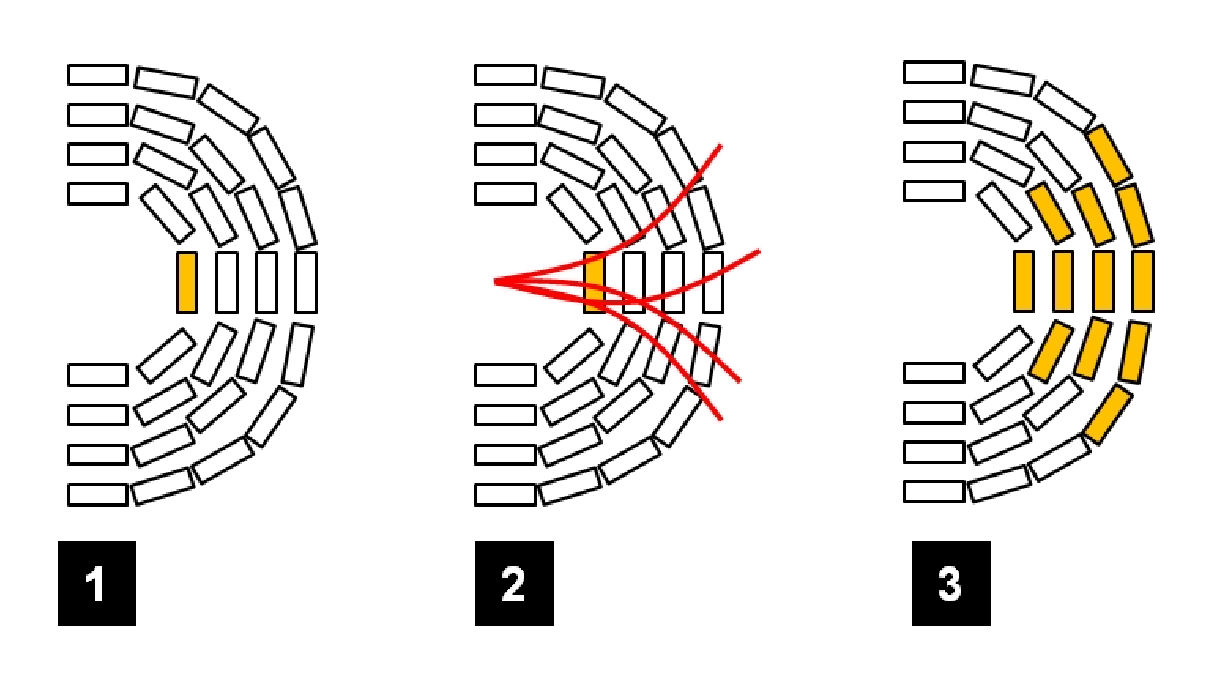
\includegraphics[width=0.6\columnwidth]{Plots/SectorDefinition.eps}
\caption{The sector definition procedure.}
\label{fig:sector_def}
\end{figure}

\begin{enumerate}
\item We start from a module of the innermost layer we want to use in the trigger.
\item We select all particles in both samples which are crossing that module.
\item The sector is formed from all the modules crossed by the selected particles in the other layers. 
\end{enumerate}  

\noindent For $\eta$ the procedure follows the same method, the particles are produced with $0<\eta<2.2$, $-15~cm<z_0<15~cm$ and $-1~mm<d_0<1~mm$.

\noindent Using this topological procedure one defines larger sectors than using simple angular consideration, in particular in outer radii. The main advantage of this method is that as there is no overlap in the innermost layers, therefore all patterns are unique. The main disadvantage is that the overlaps in the outer layers are larger than with the angular solution. This could become a problem for data distribution. In any case, the bank generation procedure is the same for both sector types. 

\subsection{Patterns definition}

\subsubsection{Pattern definition}

\noindent A pattern can be defined as a road in the sector. Each road may contain one or more tracks, as shown on the Fig.~\ref{fig:pattern}. 
\begin{figure}[ht!]
\centering
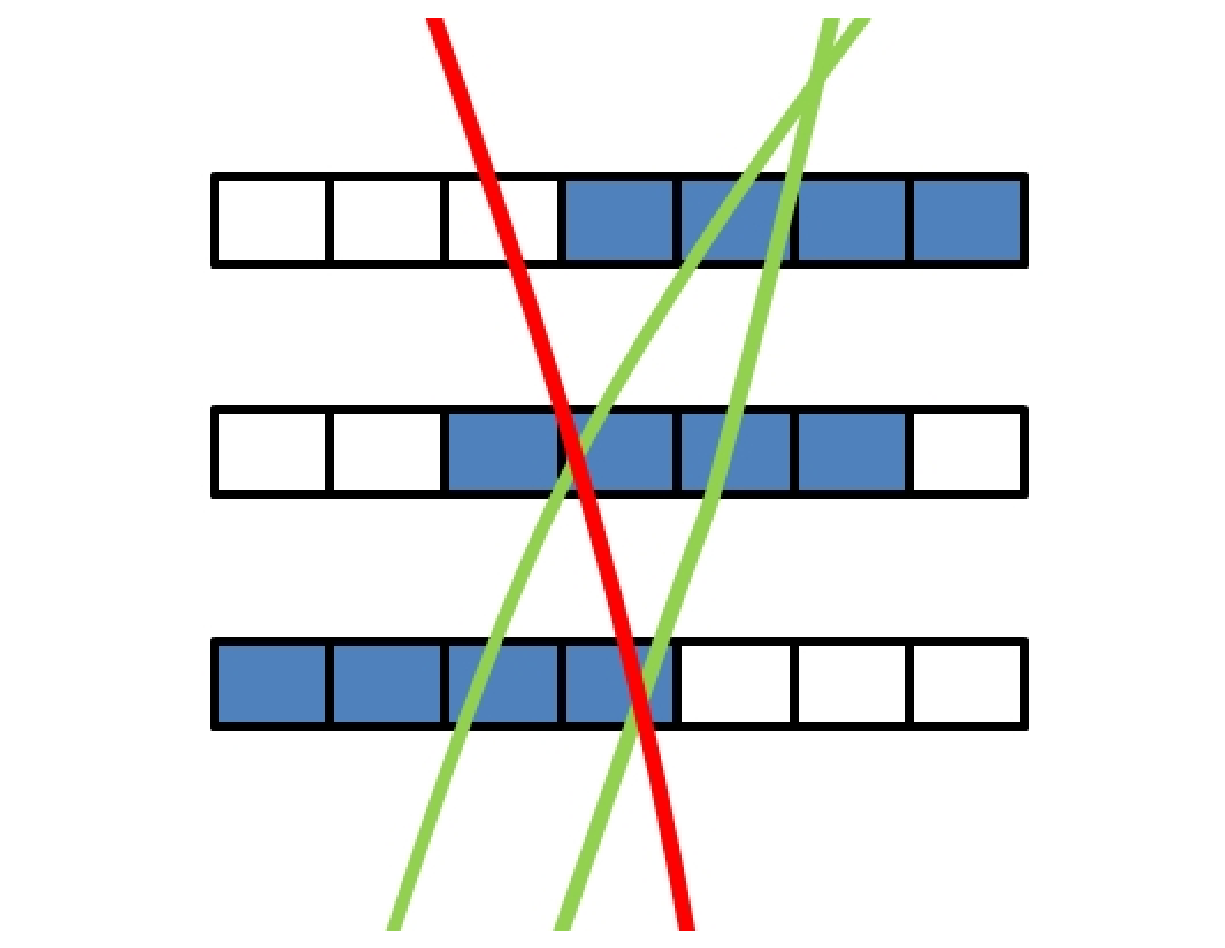
\includegraphics[width=0.3\columnwidth]{Plots/Pattern.eps}
\caption{A pattern in a three-layers detector. Green tracks will match the pattern, red tracks won't.}
\label{fig:pattern}
\end{figure}

\noindent On this picture one also get an idea of the pattern structure. Each pattern is made of one superstrip per layer. A superstrip is a group of strips/pixels, and is therefore heavily constrained by the detector itself. Once the superstrip definition has been set, its position information is coded in a N-bits word: the superstrip address. It is important to realize that the AM-based pattern recognition is using these addresses, and is therefore completely independent from the detector geometry.

\noindent As the addresses are transmitted to the AM independently for each layer, layer number doesn't have to be in the address word. In order to understand the address definition, Fig.~\ref{fig:sstrip_def} shows how a superstrip is defined in the barrel part of the tracker.  
\begin{figure}[ht!]
\centering
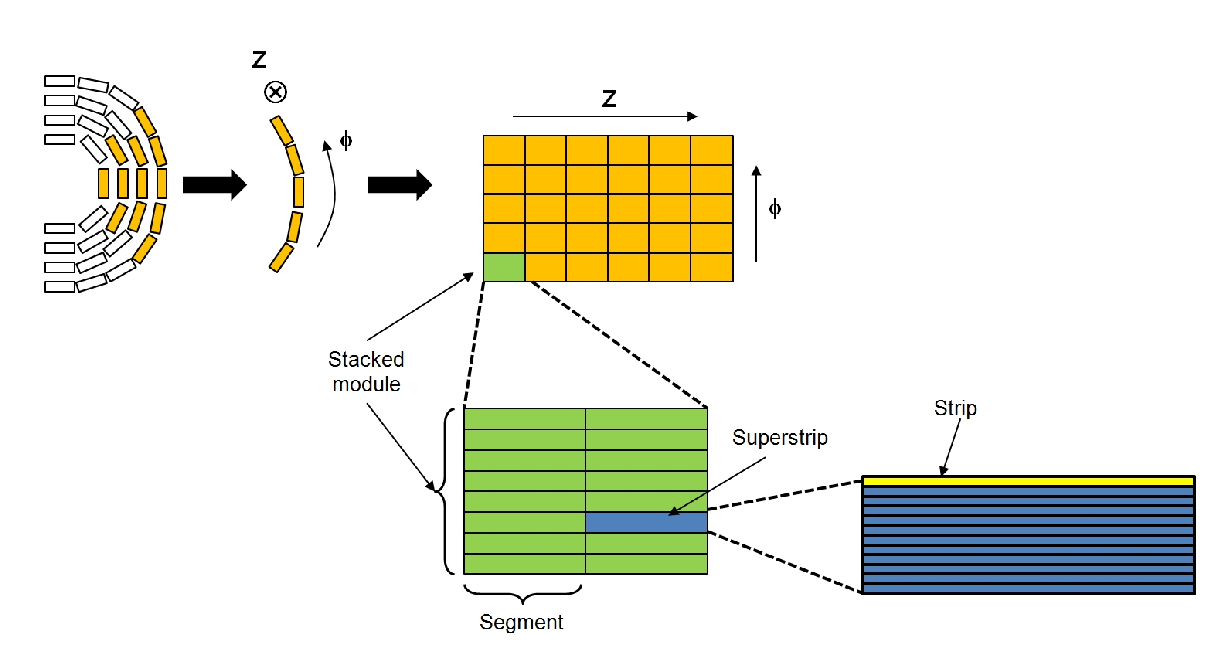
\includegraphics[width=0.7\columnwidth]{Plots/SStripDef.eps}
\caption{Geometric definition of a superstrip (barrel example).}
\label{fig:sstrip_def}
\end{figure}
\begin{figure}[ht!]
\centering
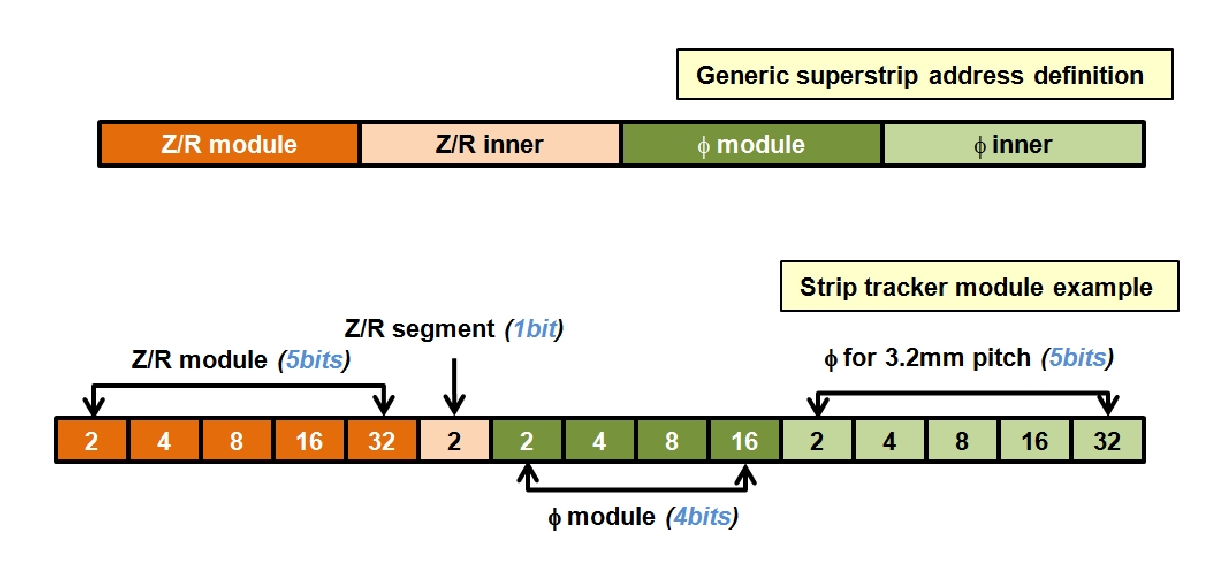
\includegraphics[width=0.7\columnwidth]{Plots/SSaddress.eps}
\caption{Address definition of a superstrip.}
\label{fig:SS_code}
\end{figure}

\noindent One has to be able to define a unique address to define the $z (resp. r)/\phi$ position of each superstrip in the barrel (resp. endcap) sector (r (resp. z) is given by the layer (resp. disk). The coding is sketched on Fig.~\ref{fig:SS_Code}. The number of bits necessary reflects the superstrip granularity and is constrained by the maximal word size acceptable by the AM chip (currently 16 bits). A first set of bits provides the module number along the corresponding coordinate: 5 bits for $Z$ (one could have up to 24 modules in Z in one sector) and 4 for $\phi$ (up to 11 modules per sector in the outermost layer). Then, for each coordinates, a second serie of bits provide the superstrip position within the module. Fig.~\ref{fig:sstrip_def} shows a tracker strip module (in green), divided into 2 segments in $Z$ and 1024 strip in $\phi$. Therefore in order to describe all the position, one would need only 1 bit for $Z$, and 10 bits for $\phi$. In practice, a certain number of strips are grouped to form the superstrip, in our case 32, thus leading to 5 in the address.   

\noindent For the endcap the coding is the same. z is just replaced by r (equivalence is made between disks and layers, ladders and rings). 


\clearpage
